%% LyX 2.1.4 created this file.  For more info, see http://www.lyx.org/.
%% Do not edit unless you really know what you are doing.
\documentclass[english]{article}
\usepackage{charter}
\renewcommand{\familydefault}{\rmdefault}
\usepackage[T1]{fontenc}
\usepackage[utf8]{luainputenc}
\usepackage{babel}
\usepackage{float}
\usepackage{graphicx}
\usepackage{setspace}
\PassOptionsToPackage{normalem}{ulem}
\usepackage{ulem}
\onehalfspacing
\usepackage[unicode=true,
 bookmarks=true,bookmarksnumbered=false,bookmarksopen=false,
 breaklinks=false,pdfborder={0 0 1},backref=false,colorlinks=false]
 {hyperref}
\hypersetup{pdftitle={How People Are Entertained: The Consequences of the 1983 Video Game Crash},
 pdfauthor={Hal Motley},
 pdfsubject={Technology},
 pdfkeywords={Atari, Video-Game-Crash, NES, unofficial, cartridges, open-console.}}

\makeatletter

%%%%%%%%%%%%%%%%%%%%%%%%%%%%%% LyX specific LaTeX commands.
\providecommand{\LyX}{\texorpdfstring%
  {L\kern-.1667em\lower.25em\hbox{Y}\kern-.125emX\@}
  {LyX}}

%%%%%%%%%%%%%%%%%%%%%%%%%%%%%% User specified LaTeX commands.
\date{}

\makeatother

\begin{document}

\title{\textbf{How People Are Entertained:}{\Large{}}\\
{\Large{}The Consequences of the 1983 Great Video Game Crash}}


\author{\textsc{Hal Motley}}

\maketitle
\begin{center}
{\large{}2\textsuperscript{nd} Edition}
\par\end{center}{\large \par}

\newpage{}


\section*{Licenses}


\subsection*{Content license}


\includegraphics[scale=1.2]{images/by-sa}\\
This document's contents, PDF file and .lyx source file are licensed
under the \textbf{Creative Commons Attribution-ShareAlike 4.0 International}
license. Full details of this license can be found here:\\
\href{http://creativecommons.org/licenses/by-sa/4.0/}{http://creativecommons.org/licenses/by-sa/4.0/}


\subsection*{In summary:}
\begin{itemize}
\item You are free to:

\begin{itemize}
\item \textit{Share} – copy and redistribute the material in any medium
or format.
\item \textit{Adapt} – remix, transform, and build upon the material for
any purpose, even commercially.
\item The licensor cannot revoke these freedoms as long as you follow the
license terms.
\end{itemize}
\item Under the following terms:

\begin{itemize}
\item \textit{Attribution} – You must give appropriate credit, provide a
link to the license, and indicate if changes were made. You may do
so in any reasonable manner, but not in any way that suggests the
licensor endorses you or your use.
\item \textit{ShareAlike} – If you remix, transform, or build upon the material,
you must distribute your contributions under the same license as the
original.
\item \textit{No additional restrictions} – You may not apply legal terms
or technological measures that legally restrict others from doing
anything the license permits.
\end{itemize}
\item Notices:

\begin{itemize}
\item You do not have to comply with the license for elements of the material
in the public domain or where your use is permitted by an applicable
exception or limitation.
\item No warranties are given. The license may not give you all of the permissions
necessary for your intended use. For example, other rights such as
publicity, privacy, or moral rights may limit how you use the material.
\end{itemize}
\end{itemize}

\subsection*{E-book license}


\includegraphics[scale=0.5]{images/PD-icon}\\
This e-book's \LaTeX{}, XHTML, CSS and XML source code are licensed
under \textbf{The Unlicense}. For more information, please refer to\href{http://unlicense.org}{http://unlicense.org}\\
\\
This is free and unencumbered software released into the public domain.\\
\\
Anyone is free to copy, modify, publish, use, compile, sell, or distribute
this software, either in source code form or as a compiled binary,
for any purpose, commercial or non-commercial, and by any means.\\
\\
In jurisdictions that recognize copyright laws, the author or authors
of this software dedicate any and all copyright interest in the software
to the public domain. We make this dedication for the benefit of the
public at large and to the detriment of our heirs and successors.
We intend this dedication to be an overt act of relinquishment in
perpetuity of all present and future rights to this software under
copyright law.\\
\\
THE SOFTWARE IS PROVIDED \textquotedbl{}AS IS\textquotedbl{}, WITHOUT
WARRANTY OF ANY KIND, EXPRESS OR IMPLIED, INCLUDING BUT NOT LIMITED
TO THE WARRANTIES OF MERCHANTABILITY, FITNESS FOR A PARTICULAR PURPOSE
AND NONINFRINGEMENT. IN NO EVENT SHALL THE AUTHORS BE LIABLE FOR ANY
CLAIM, DAMAGES OR OTHER LIABILITY, WHETHER IN AN ACTION OF CONTRACT,
TORT OR OTHERWISE, ARISING FROM, OUT OF OR IN CONNECTION WITH THE
SOFTWARE OR THE USE OR OTHER DEALINGS IN THE SOFTWARE.

\newpage{}


\section*{Preface}

This article was written back in 2013 for an assignment for my first
(and only) year of Computer Science at the University of Derby. The
assignment asked that the article be 2-3 pages long and stringently
follow the IEEE document standard (\href{https://www.ieee.org/documents/MSW_A4_format.doc}{https://www.ieee.org/documents/MSW\_{}A4\_{}format.doc}).

As someone who can't stand Times New Roman (particularly at point
size 12), I was never quite satisfied with what I submitted even when
I was happy with the content I had written and the images I had found
and provided.

So I have finally put this article where I believe it belongs; in
a \LyX{} document with attractive typesetting in a presentable serif
typeface (Charis SIL) using knowledge I have gained afterward from
book typesetting and e-book production.

I also wanted to fix up some grammatical mistakes, re-check the reference
links, do some general fixes and provide an ePub counterpart. So with
that in mind I do consider this updated version of the article to
be the superior version.

The original article I submitted was recently published and then released
to the general public via the ``Computers for Everyone'' section
of their ``Open Journal Systems @ Department of Computing \& Mathematics
@ Derby'' website. There are also plenty of other articles by fellow
students who I shared with on my course, I recommend you read them
too!\\
\href{http://computing.derby.ac.uk/ojs/index.php/c4e/article/view/90/67}{http://computing.derby.ac.uk/ojs/index.php/c4e/article/view/90/67}

\newpage{}


\section*{Article}


\subsection*{Abstract}

This document explains what led to the Great Video Game Crash in 1983.
The main consequences will then be presented, in particular, the lockdown
of consoles to unofficial games, and homebrew. Finally, the recent
successful use of the open model will be briefly reviewed.


\subsection*{Index Terms}

Atari, Video-Game-Crash, NES, unofficial, cartridges, open-console.


\subsection*{\textsc{Introduction}}

The year is 2013, video games are commonplace and the industry as
a whole seems to be prospering well (Gartner, 2013). It was not always
smooth sailing and for a short while the entire games industry's future
was put into question, after a 97\% drop in market value in 1983 during
the Atari era in the United States (CleverNoobs, 2013, 0:0:20; Electronic
Games Magazine, 1985, pp. 30-31).


\subsection*{\textsc{The Great Video Game Crash of 1983}}

The name of this huge dent on the industry was The Great Video Game
Crash of 1983. The name is used to describe the events that brought
the market value down to such a low level. It was caused by multiple
factors, which can almost be completely attributed to the Atari 2600's
openness because anyone could make cartridges for the console.

The first step towards the crash happened in 1979 when a handful of
disgruntled games developers working for Atari were unhappy that they
were not credited for each game's development and that they did not
receive royalties for each copy sold. Since Atari refused to alter
their policy to fit the games developers' demands, they left the company
to form the World's first 3\textsuperscript{rd} party publisher,
Activision (Activision, n.d.). This first step meant that not only
did Atari lose talent but they gained competition. The console's openness
meant that Activision could make and sell cartridges for the Atari
2600 without paying any license or royalties back to Atari. This was
not helpful to Atari at all and foreshadowed what was yet to come.

The second step was that Atari released some poor 1\textsuperscript{st}
party licensed titles for the 2600, both \textit{Pac-Man} and \textit{E.T.
the Extra-Terrestrial} (E.T.) which were released in 1982. They were
highly anticipated but badly received by critics and fans because
they were full of bugs and glitches and not particularly fun to play.
This was not helped by the fact they were both were rushed to completion
and lacked quality assurance by Atari. Atari had spent a great deal
of money in licensing fees for rights to \textit{E.T.} and Pac-Man,
and they got little financial gain from it when their customers realised
that these games were not worth the investment (Giant Bomb, E.T.)
(IGN, Top 10 Best-Selling Atari 2600 Games).

The third step was that many other companies were wanting to the ride
the video game money train. Back in the 1980's, video games were the
fastest growing industry in all the USA. Many companies including
Quaker, Purina and Mystique all made atrocious games to capitalise
on huge market. Though this effect pushed it down even further (CleverNoobs,
2013). With games like \textit{Chase the Chuck Wagon}, \textit{Name
this Game} and, all created by these companies purely for profit over
entertainment value.

The fourth step was that at the same as the Atari 2600 era was the
birth of the affordable personal computer which could allow the consumer
to both play games and be productive. Further adding competition to
Atari's business because there were other machines on the market that
could do multiple things for your money (CleverNoobs, 2013, 0.2.0).
With all these terrible games out there and competition from the personal
computer space, most consumers simply got tired and angry playing
with console games. So enough consumers voted with their wallets and
decided not to buy them. This caused the market to topple over and
caused the 97\% drop from \$3.2 billion (\textasciitilde{}\pounds{}2
billion) to \$100 million (\textasciitilde{}\pounds{}63 million)
almost dooming it completely (CleverNoobs, 2013, 0:0:50)\\
\begin{figure}[H]
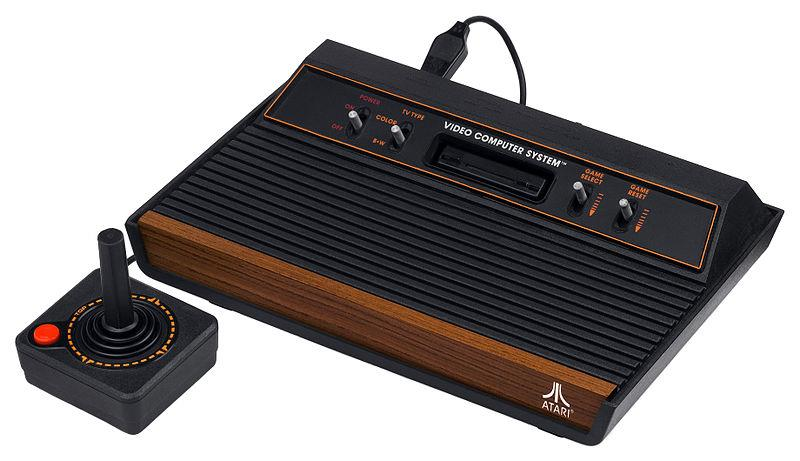
\includegraphics[scale=0.4]{images/atari2600}

\caption{Atari 2600 Console}


\end{figure}



\subsection*{\textsc{Recovery of the Console}}

The market was almost down and out, consumers were immensely cynical
of the words “video game”. If it was not for Nintendo, through some
clever marketing tactics with the advertising of Robotic Operating
Buddy (R.O.B), a peripheral for their upcoming Nintendo Entertainment
System (NES) console the console gaming industry might not have ever
been resuscitated back to its former glory.

The NES managed to bring the industry back on track, with Nintendo
learning from Atari's mistakes in the past. Nintendo saw that 3\textsuperscript{rd}
party development for their console could be beneficial to their business,
but it should be controlled with licensing (an agreement between the
publisher and the console manufacturer) to ensure both quality control
and enable Nintendo to profit off the games' sales. There were many
successful 3\textsuperscript{rd} party titles including \textit{Tetris}
(1989), \textit{Teenage Mutant Ninja Turtles} (1989) and \textit{Punch-Out!!}
(1987). Nintendo did not rest on their laurels with just 3\textsuperscript{rd}
party content and began to release games of their own much like Atari
did. Many of these games were the first entry to many loved franchises
including \textit{Super Mario Bros.} in 1985 (which itself was the
bestselling NES game of all-time), \textit{Legend of Zelda} (1986)
and \textit{Metroid} (1986). These were all well received by the audience
and, subsequently, have received many sequels to this day.

Since the NES console was locked down due to Nintendo learning from
Atari's main mistake of allowing oversaturation of content, games
that were not approved by Nintendo would be released unofficially
as cartridges but would never receive the sales figures or critical
attention that most official content would receive (IGN, n.d.). This
included games that were not even submitted to Nintendo to approve
because of content, a reluctance to pay licensing fees and a disagreement
over licensing conditions. The unofficial cartridges would often look
physically different to official cartridges and used techniques to
bypass the 10NES authorisation chip that were present in official
cartridges to ensure only official cartridges could be played (Horton
K., n.d.). In fact, Atari under a subsidiary called Tengen, actually
made unofficial cartridges for the NES as well as having their games
officially released on the console under the Atari name (Oxford, 2005).

The console continued selling until the NES's successor Super Nintendo
Entertainment System (SNES) arrived in the early 90's as the direct
successor to the NES. While it sold less units than the original NES,
it retained dominance over competition from Sega with their MegaDrive
(Genesis in the USA) and other consoles. The console itself had full
16-bit capabilities bringing improved graphical and sound capabilities
with it (Buchanan, 2009). Subsequent consoles would also be locked
down and the consumer would be prevented from playing unofficial 3\textsuperscript{rd}
party content and using unofficial 3\textsuperscript{rd} party accessories
by the manufacturers, because it was a system that was proven to work
for the console manufacturers (Chacksfield, 2010).

Whilst there were a few hobby consoles that were open to modification
by the manufacturer, such as, the Pandora console by OpenPandora,
and the Dingoo A320 by Dingoo Technology Ltd, none of these consoles
took the Internet by storm like the OUYA did. The OUYA, which is a
\$99 (\pounds{}99) microconsole using Google's Android™ platform,
received \$8,596,474 (\pounds{}5,346,069) in funding with 63,416
backers via the crowdfunding platform Kickstarter in 2012 (Kickstarter,
2012). This suggests that customers had a great deal of faith in the
concept of an open console. Furthermore the OUYA has recently celebrated
its 500\textsuperscript{th} game, that is, \textit{Neon Shadow} (Tasty
Poison Games, 2013). The OUYA is built on the foundation of being
an open system where every game is free to try out with games available
to purchase via digital distribution. In September 2013 Valve formally
announced the Steam Machine, which is an open console backed by them
which allows modification in a similar fashion to that of an ordinary
gaming PC (Valve, 2013). The fact that Valve has invested in custom
hardware for the Steam Machine itself, the controller and the operating
system, implies that they have confidence in making profit from an
open console.

This is most likely due to the extreme popularity of their digital
distribution Steam. Steam (and most other digital distributors) solved
Atari's issue back in the early 1980's, by managing quality control
via a number of methods. For example, Steam Greenlight allows the
opportunity for potential customers to vote for a game before it is
allowed to be sold on the storefront.\\
\begin{figure}[H]
\begin{centering}
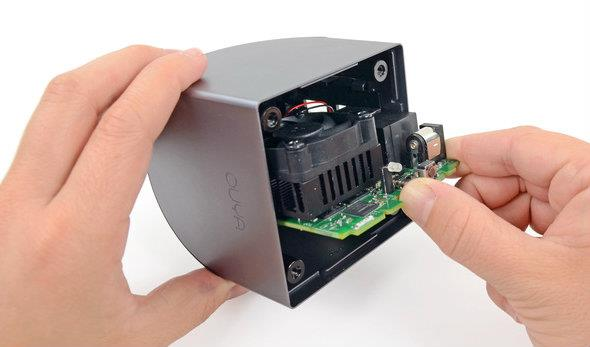
\includegraphics[scale=0.4]{images/ouya}
\par\end{centering}

\caption{OUYA Console}


\end{figure}
\begin{figure}[H]
\begin{centering}
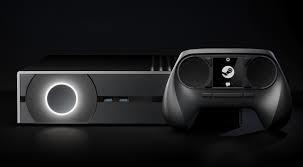
\includegraphics{images/steammachine}
\par\end{centering}

\caption{Steam Machine Concept}
\end{figure}
\newpage{}


\section*{Bibliography}


\subsection*{References}

References for the main text are listed alphabetically by author rather
than chronologically:
\begin{enumerate}
\item \textbf{Activision} (n.d.)\textit{ Historical Timeline} (online)\\
Available at: \sout{http://investor.activision.com/timeline.cfm}
(dead link), archive available at: \href{http://web.archive.org/web/20131018030348/http://investor.activision.com/timeline.cfm}{http://web.archive.org/web/20131018030348/http://investor.activision.com/timeline.cfm}\\
(Last date accessed: 13\textsuperscript{th} February 2018)
\item \textbf{Buchanan, L.}(2009)\textit{ Genesis vs. SNES: By the Numbers}
(online)\\
Available at:\href{http://uk.ign.com/articles/2009/03/20/genesis-vs-snes-by-the- numbers}{http://uk.ign.com/articles/2009/03/20/genesis-vs-snes-by-the- numbers}\\
(Last date accessed: 12\textsuperscript{th} March 2015)
\item \textbf{Chacksfield, M.} (2010)\textit{ Nintendo DS R4 cards declared
illegal in UK} (online)\\
Available at:\href{http://www.techradar.com/news/gaming/nintendo-ds-r4-cards- declared-illegal-in-uk-706317}{http://www.techradar.com/news/gaming/nintendo-ds-r4-cards- declared-illegal-in-uk-706317}\\
(Last date accessed: 12\textsuperscript{th} March 2015)
\item \textbf{CleverNoobs}(2013)\textit{ Is the Gaming Industry Crashing?}(online)\\
Available at:\href{http://www.youtube.com/watch?v=XZxXEidtxHk}{http://www.youtube.com/watch?v=XZxXEidtxHk}\\
(Last date accessed: 12\textsuperscript{th} March 2015)
\item \textbf{Gartner} (2013)\textit{ Gartner says Worldwide Video Game
Market to Total \$93 billion in 2013} (online)\\
Available at:\href{http://www.gartner.com/newsroom/id/2614915}{http://www.gartner.com/newsroom/id/2614915}\\
(Last Accessed: 12\textsuperscript{th} March 2015)
\item \textbf{Horton, K.} (n.d.)\textit{ The Infamous Lockout Chip} (online)\\
 Available at:\href{http://www.kevtris.org/mappers/lockout/}{http://www.kevtris.org/mappers/lockout/}\\
(Last date accessed: 12\textsuperscript{th} March 2015)
\item \textbf{IGN} (n.d.)\textit{ Top 100 NES Games}. (online) IGN Entertainment
Ltd.\\
Available at:\href{http://uk.ign.com/top-100-nes-games/}{http://uk.ign.com/top-100-nes-games/}\\
(Last date accessed: 12\textsuperscript{th} March 2015)
\item \textbf{Katz, A.} (1985) \textit{1984: The Year That Shook Electronic
Gaming}. Electronic Games Magazine.\\
 (January, pp 30-31) NY: Reese Communications Ltd.
\item \textbf{Kickstarter} (2012)\textit{ OUYA: A New Kind of Video Game
Console} (online)\\
Available at:\href{http://www.kickstarter.com/projects/ouya/ouya-a-new-kind-of-video-game-console}{http://www.kickstarter.com/projects/ouya/ouya-a-new-kind-of-video-game-console}\\
(Last date accessed: 12\textsuperscript{th} March 2015)
\item \textbf{Oxford, N.} (2005)\textit{ Trials \& Tribulations: Video games
many visits to court.} (online)\\
Originally available at: \sout{http://www.1up.com/features/trials-and-tribulations?pager.offset=1}
(dead link), archive available at: \href{https://web.archive.org/web/20131017023035/http://www.1up.com/features/trials-and-tribulations?pager.offset=1}{https://web.archive.org/web/20131017023035/http://www.1up.com/features/trials-and-tribulations?pager.offset=1}\\
 (Last date accessed: 13\textsuperscript{th} February 2018)
\item \textbf{Tasty Poison Games} (2013)\textit{ Neon Shadow 500th game
on OUYA!} (online)\\
Available at:\href{http://tastypoisongames.com/2013/11/neon-shadow-500th-game-ouya/}{http://tastypoisongames.com/2013/11/neon-shadow-500th-game-ouya/}\\
(Last date accessed: 12\textsuperscript{th} March 2015)
\item \textbf{Valve} (2013)\textit{Steam Machines} (online)\\
Available at:\href{http://store.steampowered.com/livingroom/SteamMachines/}{http://store.steampowered.com/livingroom/SteamMachines/}\\
(Last Accessed: 12\textsuperscript{th} March 2015)
\end{enumerate}

\subsection*{List of Sources for Images}
\begin{enumerate}
\item \textbf{Amos, E.} (2011)\textit{ An Atari 2600 four-switch \textquotedbl{}wood
veneer\textquotedbl{} version, dating from 1980-1982}. (online)\\
 Available at:\href{http://en.wikipedia.org/wiki/File:Atari-2600-Wood-4Sw-Set.jpg}{http://en.wikipedia.org/wiki/File:Atari-2600-Wood-4Sw-Set.jpg}\\
(Last date accessed: 12\textsuperscript{th} March 2015)
\item \textbf{Listdium} (n.d.)\textit{ Super Fast Processor} (online)\\
Available at:\href{http://www.listedium.com/features-of-ouya-android-based/}{http://www.listedium.com/features-of-ouya-android-based/}\\
(Last date accessed: 12\textsuperscript{th} March 2015)
\item \textbf{Hollister, S.} (2013)\textit{ We Play With the Steam Machine,
Valve's Game Console of the Future} (online)\\
Available at:\href{http://www.theverge.com/2013/11/4/5063760/we-try-the-steam-machine-valves-video-game-console-of-the-future}{http://www.theverge.com/2013/11/4/5063760/we-try-the-steam-machine-valves-video-game-console-of-the-future}\\
(Last date accessed: 12\textsuperscript{th} March 2015)\end{enumerate}

\end{document}
